% ---
\documentclass{article}


% Packages
% ---
\usepackage{amsmath,amssymb,amsthm} 	% Advanced math typesetting
% \usepackage[utf8]{inputenc} 	% Unicode support (Umlauts etc.)
\usepackage[USenglish]{babel} 	% Change hyphenation rules
\usepackage{hyperref} 				% Add a link to your document
\usepackage{graphicx}				% Add pictures to your document
\graphicspath{ {./images/} }	% image directory
\usepackage{listings} 				% Source code formatting and highlighting
\lstset{basicstyle=\ttfamily}		%Typewriter font for code writing
\usepackage{geometry}
\geometry{margin=1in}
\usepackage{enumitem}
\usepackage{float}
%\floatstyle{boxed}
\restylefloat{figure}
\usepackage{mathabx}
\usepackage{fancyhdr}
\usepackage[dvipsnames]{xcolor}

\theoremstyle{definition}
\newtheorem{definition}{Def}

\pagestyle{fancy}
\fancyhf{}
\lhead{\bf CPSC 340 \\ Week 2 }
\rhead{\bf Jeremi Do Dinh \\ 61985628}
\rfoot{Page \thepage}



\usepackage{tikz}						% Graph drawing tools
\usetikzlibrary {positioning}

\usepackage{breqn}
\usepackage{multicol} 				% Multiple column functionality
\usepackage{blindtext}


\begin{document}

\noindent \url{https://www.cs.ubc.ca/~fwood/CS340/}

\section*{Lecture IV}
\textbf{January 13th, 2020}\\
\noindent \url{https://www.cs.ubc.ca/~fwood/CS340/lectures/L4.pdf}


\subsection*{Supervised Learning: Determine Home city}
\begin{itemize}
	\item We are given data from 248 homes
	\item For each home/example we have these features:
	\begin{itemize}
		\item Elevation
		\item Year
		\item Bathrooms
		\item Bedrooms
		\item Price
		\item Square feet
	\end{itemize}
\item Goal is to build a program that predicts {\bf SF} of {\bf NY}
\end{itemize}
\begin{figure}[H]
	\centering
	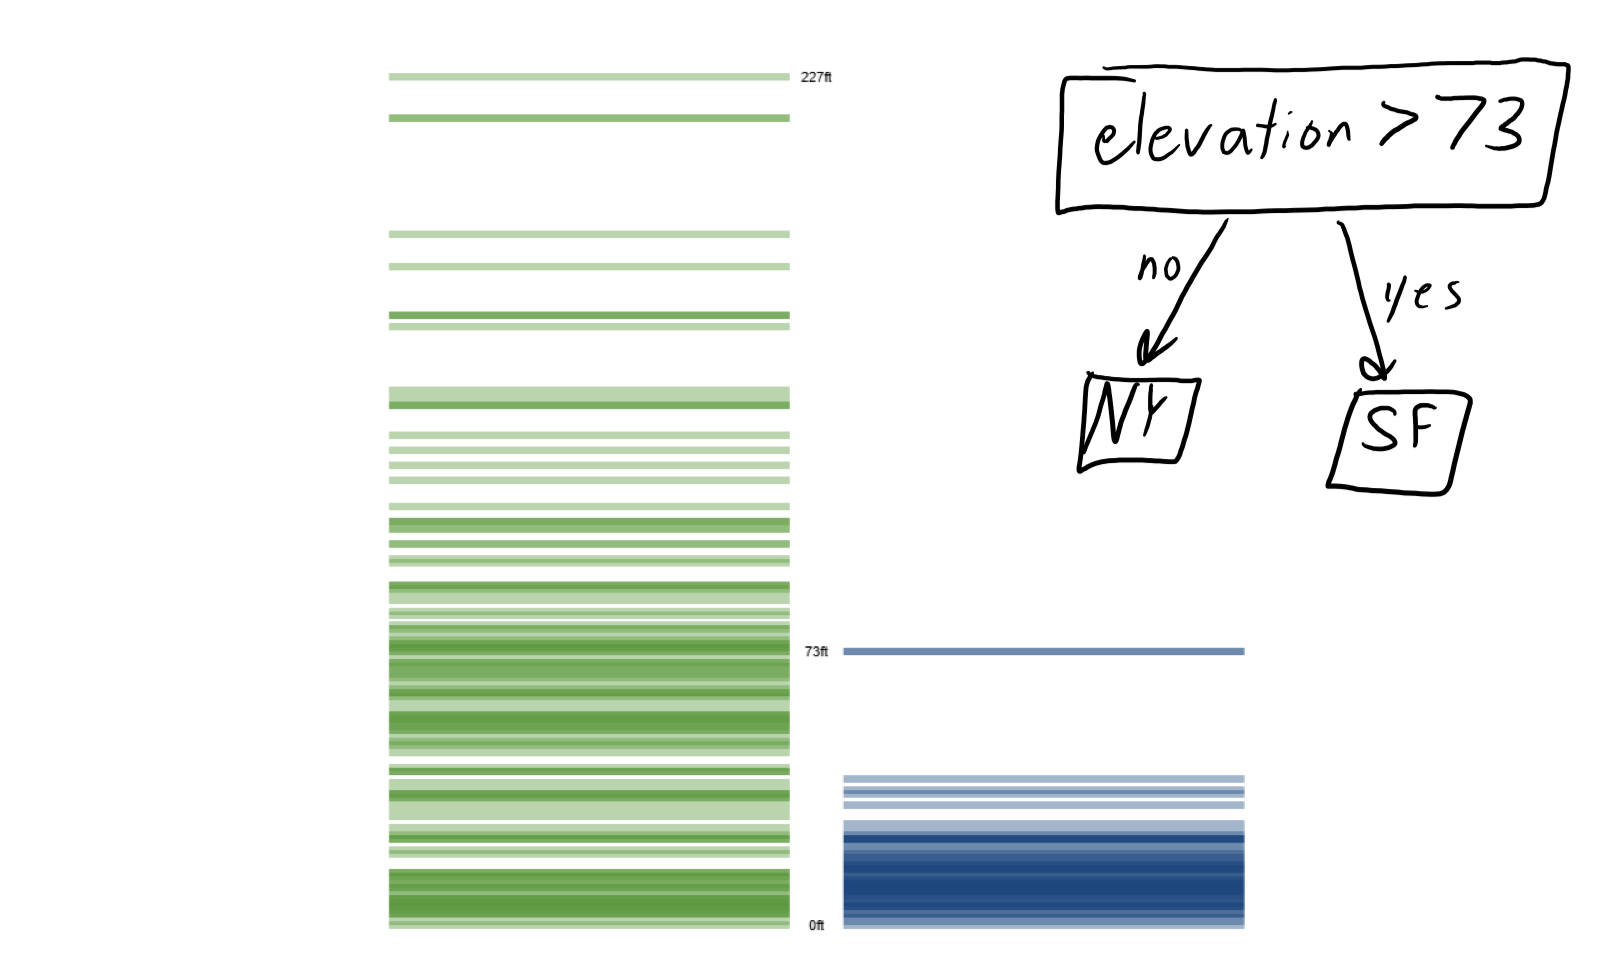
\includegraphics[width = 5in]{Pic1}
	\caption{Plotting Elevation, and consequent simple decision stump}
\end{figure}

\begin{figure}[H]
	\centering
	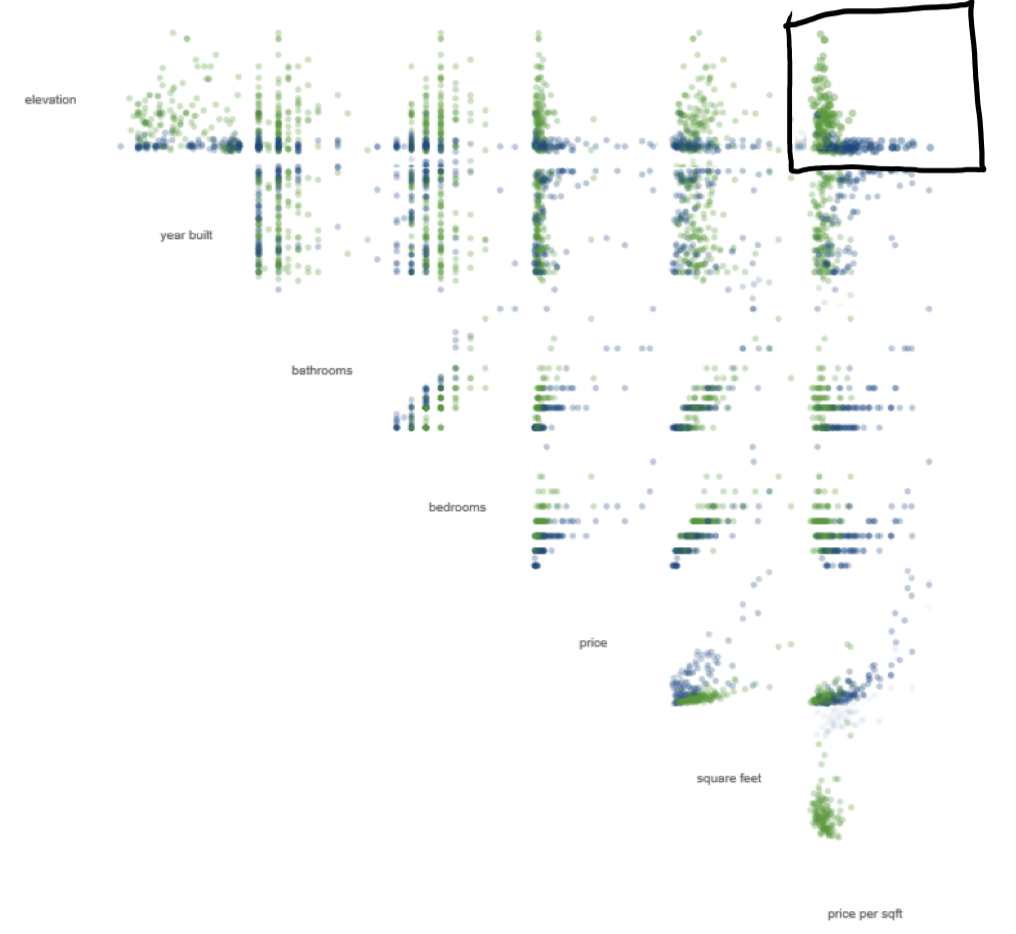
\includegraphics[width = 4in]{Pic2}
	\caption{Scatterplot array, and best visible correlation}
	
	
\end{figure}
\begin{figure}[H]
	\centering
	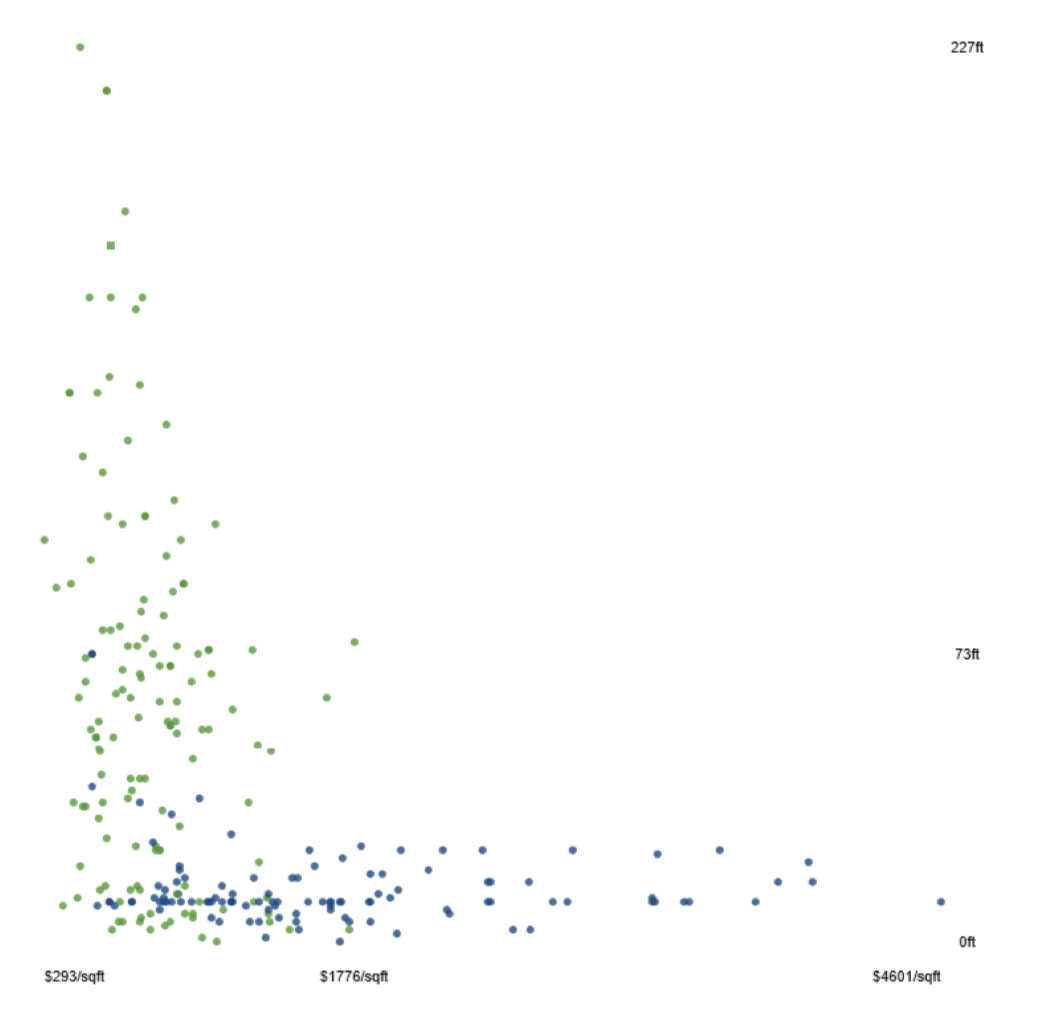
\includegraphics[width = 4in]{Pic3}
	\caption{Plotting elevation vs. Price/SqFt}
\end{figure}
\begin{figure}[H]
	\centering
	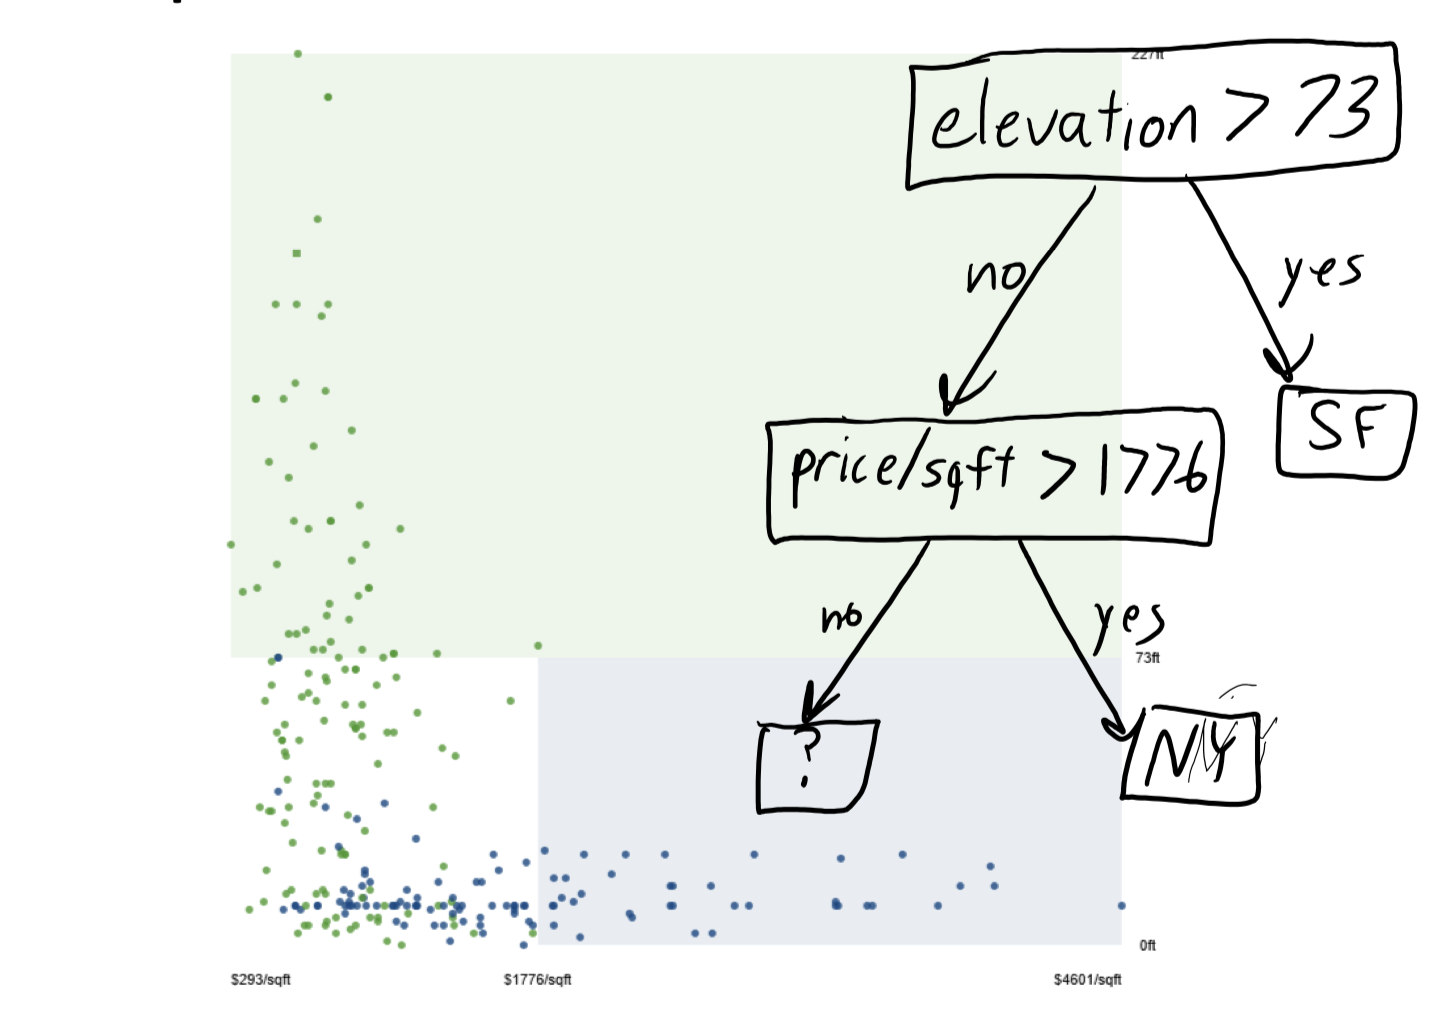
\includegraphics[width = 5in]{Pic4}
	\caption{Simple decision tree classification}
\end{figure}

\subsection*{How does Depth affect accuracy?}
We can add depth to the decision tree by splitting the data recursively. Accuracy keeps increasing as we add depth, and eventually, we can perfectly classify all of our data:
\begin{figure}[H]
	\centering
	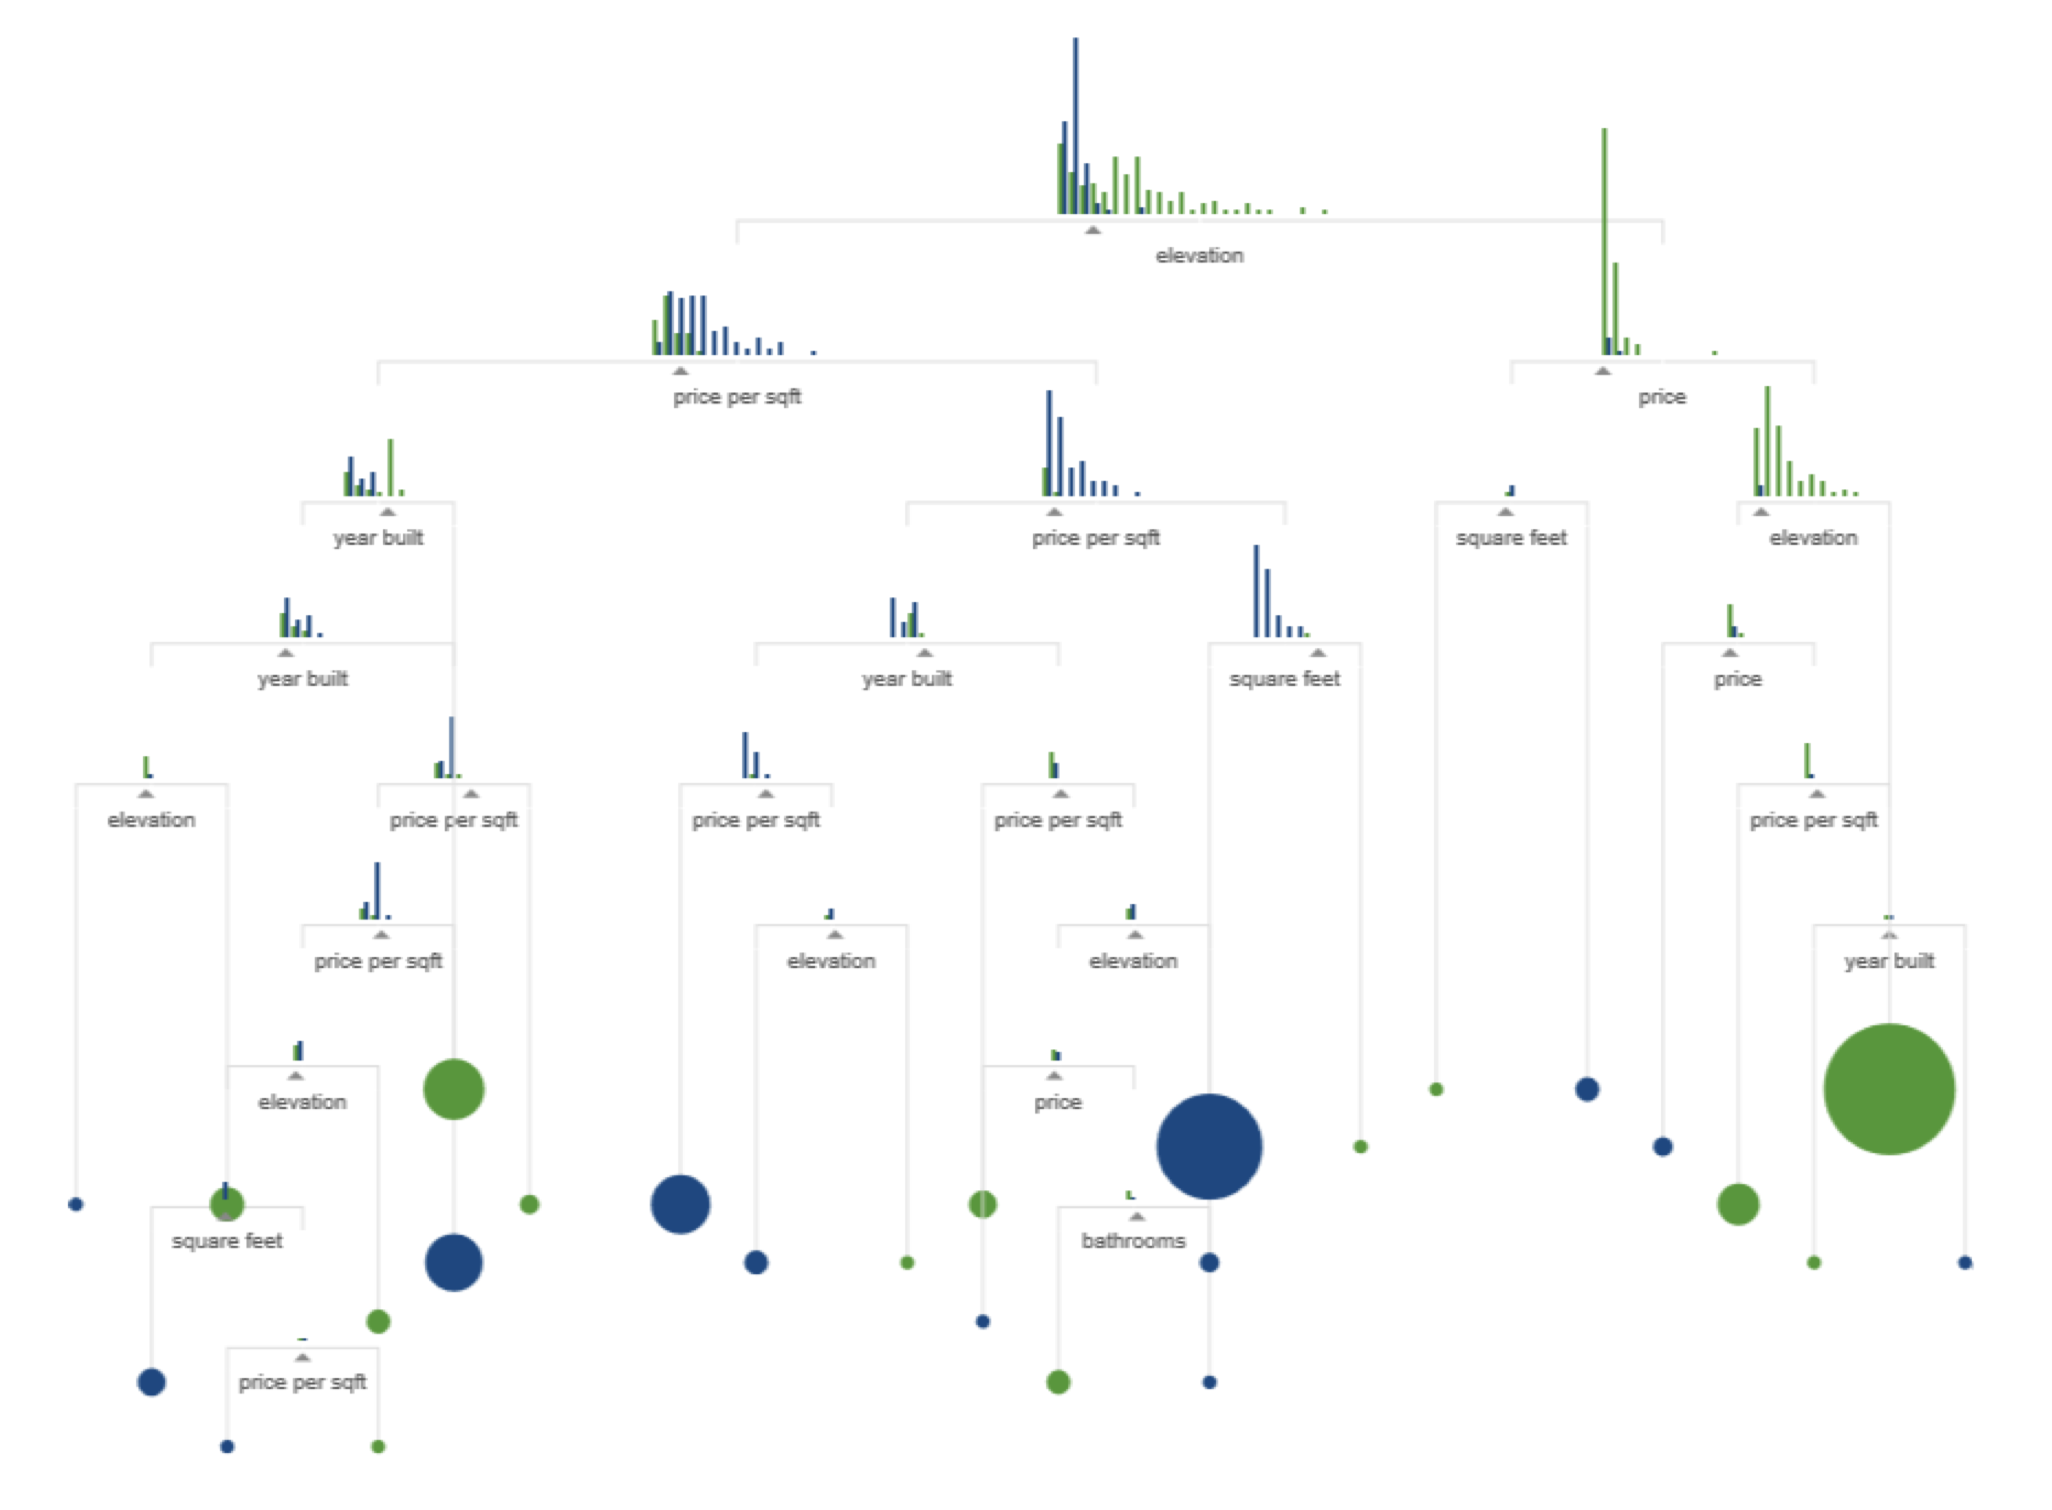
\includegraphics[width = 5in]{Pic5}
	\caption{Deep decision tree with perfect accuracy}
\end{figure}
With this decision tree, the \textsl{training accuracy} is 1. It perfectly labels the data we used to make the tree.

If we are now given 217 new homes, what is the 'testing accuracy' on the new data?
\begin{figure}[H]
	\centering
	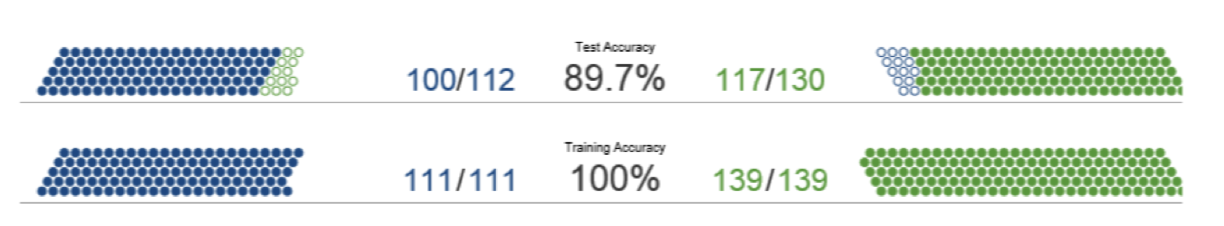
\includegraphics[width = 6in]{Pic6}
	\caption{Testing accuracy on data not used to train}
\end{figure}

\subsection*{Supervised learning notation}
\begin{itemize}
	\item We are given {\bf training data} of which we know the label:
	\begin{figure}[H]
		\centering
		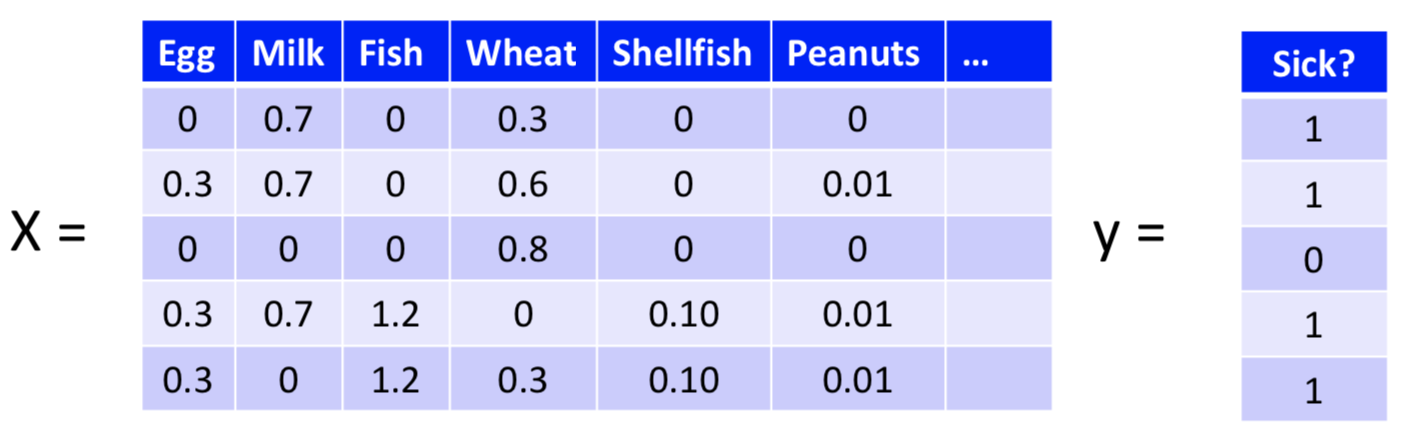
\includegraphics[width = 5in]{Pic7}
	\end{figure}
	\item We are given {\bf testing data} of which we wish to know the label
	\begin{figure}[H]
		\centering
		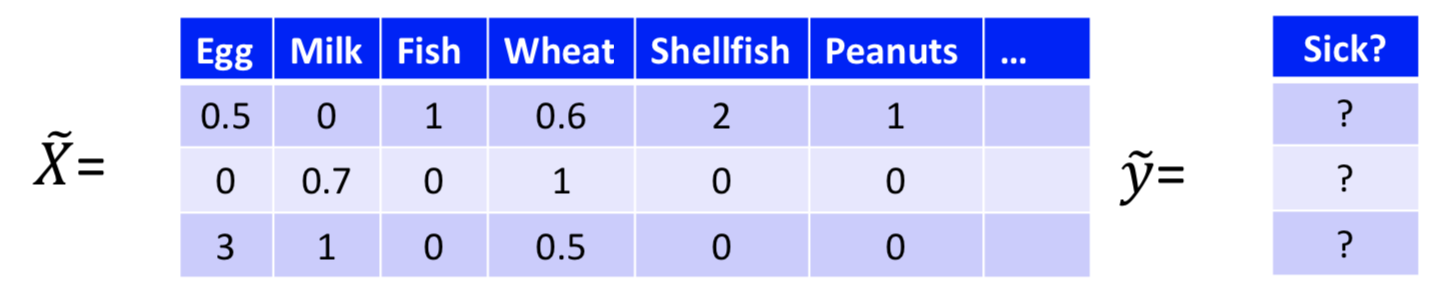
\includegraphics[width = 5.25in]{Pic8}
	\end{figure}
\end{itemize}
The typical steps are:
\begin{enumerate}
	\item Build model based on training data $ X $ and $ y $ (training phase).
	\item Model makes predictions $ \hat{y} $ on test data $ \tilde{X} $  (testing phase).
\end{enumerate}
Instead of training error, we consider test error. Are the prediction labels $\hat{y}$ similar to the true labels $\tilde{y}$

\subsubsection*{The goal of Machine Learning}
All we care about is the testing error! \\
Midterm analogy:
\begin{itemize}
	\item The training error is the practice midterm
	\item The test error is the actual midterm
	\item Goal: do well on the actual midterm, not the practice one
\end{itemize}

\subsection*{Golden rule of Machine learning}
Even though we care about the test data, \textsl{\textbf{THE TEST DATA CANNOT INFLUENCE THE TRAINING PHASE IN ANY WAY}}\\
We’re measuring test error to see how well we do on new data. If it is used in training, this isn't measured. You can start to overfit if you use it during training. 

\subsubsection*{Digression: Golden rule and hypothesis testing}
Note that the golden rule applies to hypothesis testing in scientific studies: the data you collect cannot influence the hypothesis that you test. \\
This is extremely common, and a major problem coming in many forms:
\begin{itemize}
	\item Collect huge amounts of data until you coincidentally get the significance level you want
	\item Try different ways to measure performance, and use the one that \textsl{looks} best
	\item Choose a different type of model/hypothesis after looking at the data
\end{itemize}
{\bf In general:} if you want to modify your hypotheses, you need to try on new data, or at least be aware and honest about the issue when reporting the findings. 

\subsection*{Is learning possible?}
In general, training error doesn't give us any information about testing error. The test data might have absolutely nothing to do with the training data. Thus, in order to learn, we need \textsl{assumptions}:
\begin{itemize}
	\item The training and test data must be related in some way
	\item Most common assumption: \textsl{\textbf{Independent and Identically Distributed (IID)}}
\end{itemize}

\subsection*{IID Assumption}
Training/test data is \textsl{independent and identically distributed (IID)} if:
\begin{itemize}
	\item All examples come from the same distribution (identically distributed)
	\item The examples are sampled independently (order doesn't matter)
\end{itemize}
\subsubsection*{Ex: IID in the food allergy example}
Is the food allergy example IID:
\begin{itemize}
	\item Do all the examples come from the same distribution?
	\item Does the order of the examples matter?
\end{itemize}
\textbf{\textsl{NO!}}
\begin{itemize}
	\item Being sick might depend on what you ate yesterday! (Not independent)
	\item Your eating habits might've changed over time (Not identically distributed)
\end{itemize}

\subsection*{Learning Theory}
The IID assumption makes learning possible because pattern in the training examples are likely to be similar to the ones in the testing examples. But the IID assumption is \textsl{rarely true}:
\begin{itemize}[label=-]
	\item It is a good approximation
	\item There are other possible assumptions
\end{itemize}
Also, we're assuming IID across examples, and not the features.\\
\textsl{\textbf{Learning Theory}} explores how training error is related to test error. We'll look at a few simple examples, using this notation:
\begin{itemize}
	\item $ E_{\text{train}} $ is the error in the training data
	\item $ E_{\text{test}} $ is the error in the testing data
\end{itemize}
\subsection*{Fundamental Trade-Off}
\begin{align*}
	E_{\text{test}} &= E_{\text{test}} \\
E_{\text{test}} &= (E_{\text{test}} - E_{\text{train}}) + E_{\text{train}} \\
E_{\text{test}} &= E_{\text{approx}} + E_{\text{train}} 
\intertext{where:}
E_{\text{approx}} &= E_{\text{test}} - E_{\text{train}}
\end{align*}
If $ E_{\text{approx}} $ is small, the $ E_{\text{train}} $ is a good approximation to $ E_{\text{test}} $, and $ E_{\text{approx}} $ is the "amount of over fitting":
\begin{itemize}
	\item It gets smaller as $ n $ get larger
	\item It tends to grow, as the model gets more complicated
\end{itemize}
This leads to a \textsl{{\bf fundamental trade off}}:
\begin{itemize}
	\item $ E_{\text{train}} $: How small can you make training error
	\item $ E_{\text{approx}} $: How well the training error approximates the test error
\end{itemize}
In \textsl{\textbf{simple models}} for instance (like decision stumps):
\begin{itemize}[label=-]
	\item $ E_{\text{approx}} $ is low (since it is not very sensitive to the training set), but $ E_{\text{train}} $ might be high
\end{itemize}
However in \textbf{\textsl{complex models}} (like deep decision trees):
\begin{itemize}[label=-]
	\item $ E_{\text{train}} $ may be low, but $ E_{\text{approx}} $ may be high (since it is very sensitive to the training set)
\end{itemize}
\textsl{In general}:
\begin{itemize}
	\item Training error is high for low depth (\textsl{underfitting})
	\item Training error gets better with depth
	\item Test error initially goes down, but eventually increases (\textsl{overfitting})
\end{itemize}
\begin{figure}[H]
	\centering
	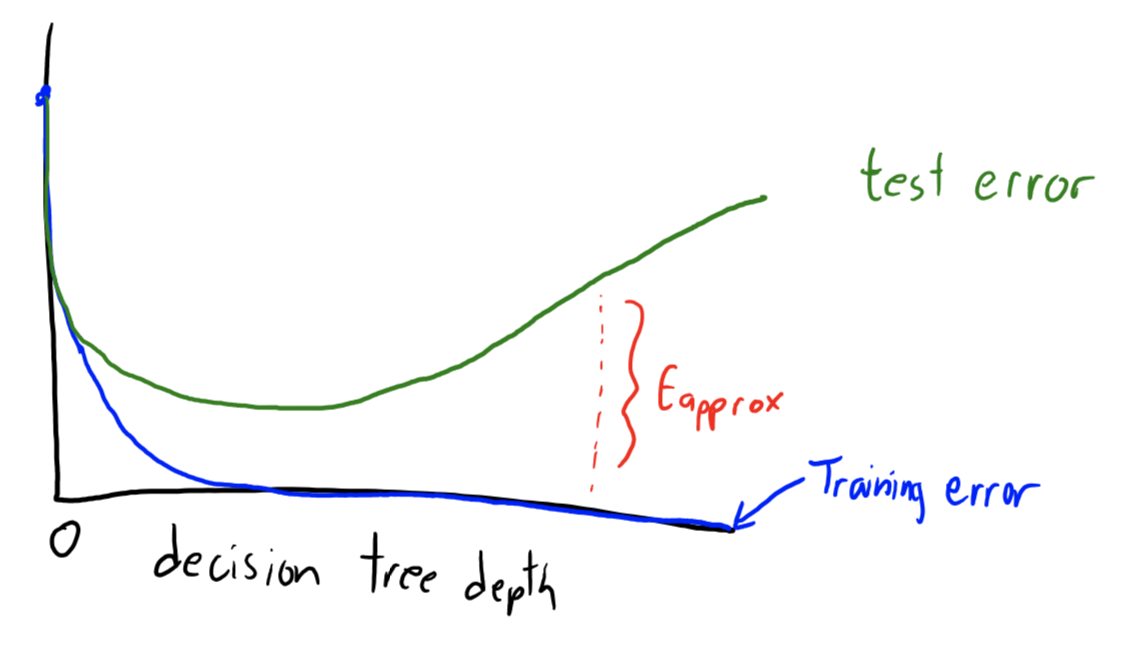
\includegraphics[width = 4in]{Pic9}
	\caption{Effect of tree depth on approximation error}
\end{figure}

\subsection*{Validation Error}
Questions at this point may be:
	\begin{itemize}
		\item How do we decide decision tree depth?
		\item We care about the test error, but we can't look at the test data!?
		\item So what do we do???
	\end{itemize}
\textbf{One answer}: We can look at the testing data to approximate test error. This consists of splitting the training examples into a \textsl{training set} and a \textsl{validation set}:

\begin{itemize}
	\item \textcolor{OliveGreen}{Train model based on training data}
	\item \textcolor{OliveGreen}{Test model based on validation data}
\end{itemize}
\begin{figure}[H]
	\centering
	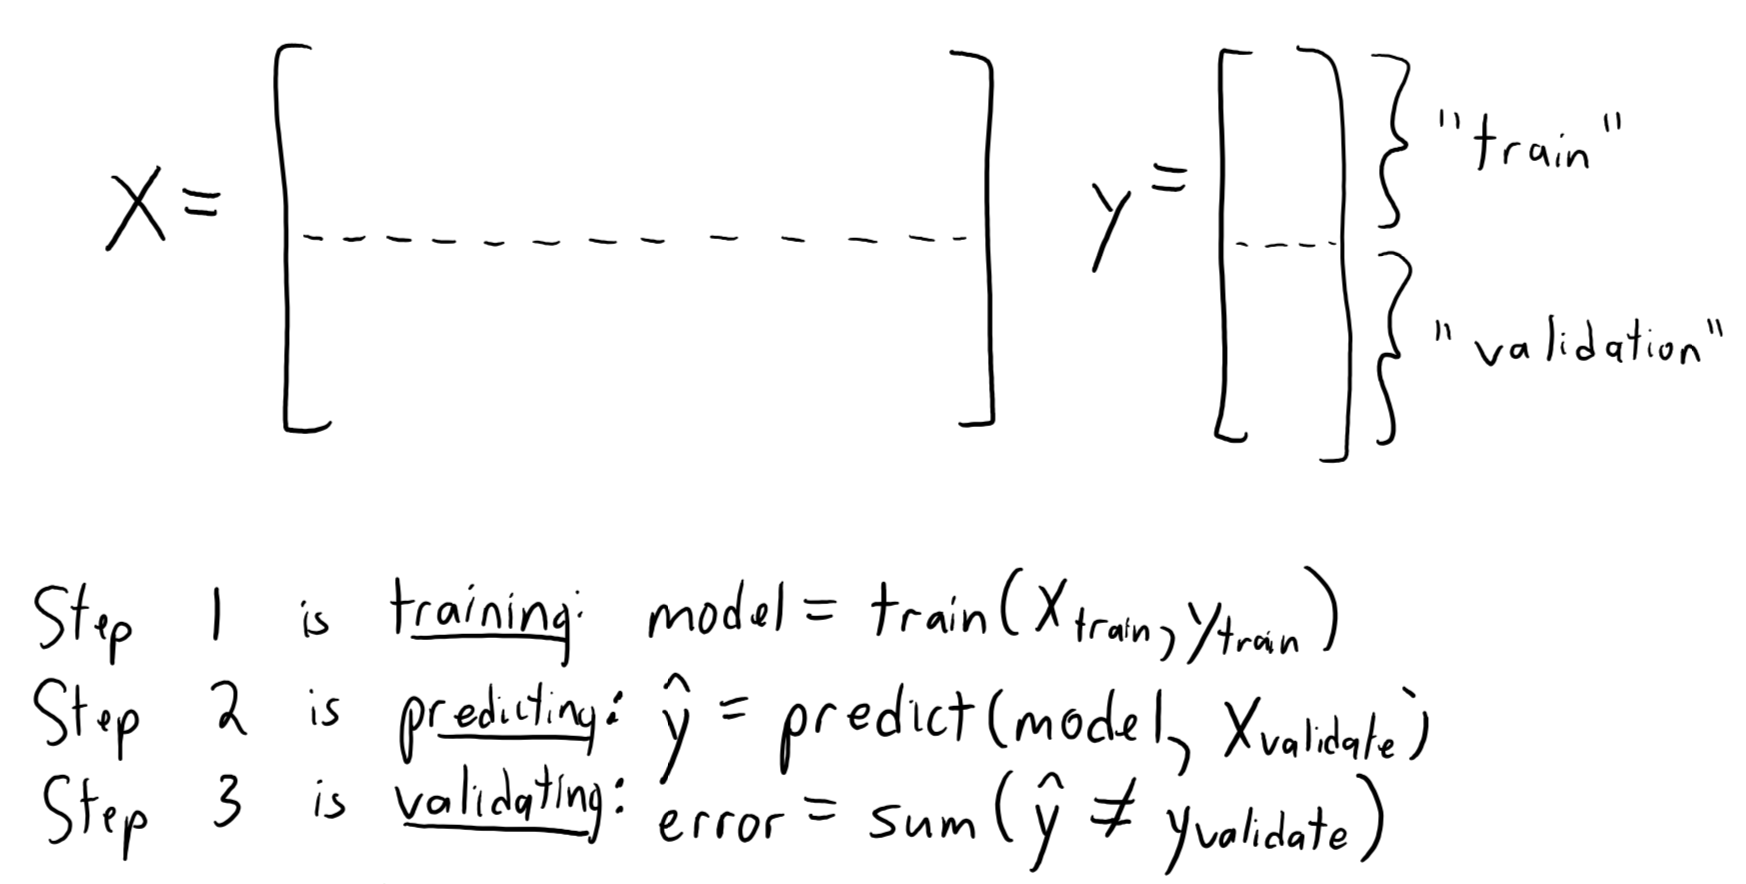
\includegraphics[width = 4.5in]{Pic10}
\end{figure}
For IID data: validation error is the unbiased approximation of test error:
\begin{align*}
	\mathbb{E}(E_{\text{valid}}) = \mathbb{E}(E_{\text{test}})
\end{align*}
\textbf{Midterm analogy}
\begin{itemize}
	\item You have 2 practice midterms
	\item You hide one midterm, and spend a lot of time working through the other
	\item You then do the other practice term, to see how well you’ll do on the test
\end{itemize}
The validation error is then chosen to choose the "\textsl{Hyper-parameters}"

\subsubsection*{Notation: Parameters and Hyper-parameters}
\begin{enumerate}
	\item The decision tree \textbf{rule} values are called the \textbf{parameters}. They control how well we fit the data set. We train the model to find the best parameters on training data.
	\item The decision tree \textbf{depth} is called a \textbf{hyper-parameter}. It controls how \textsl{complex} our model is. We \textsl{can't train} a hyper parameter, however we \textsl{validate} a hyper parameter using a validation score
\end{enumerate}
\subsubsection*{Choosing hyper-parameters with a validation set}
To choose a good value of depth (hyper parameter), we could try decision trees of different depth (say 1 to 20), and compute the validation error for each. We return the depth with the lowest validation error. \\
After this hyper-parameter is chosen, we re-train on the whole training set, with the chosen hyper-parameter. 
\subsection*{Optimization Bias}
Another name for overfitting is \textbf{optimization bias}. How biased is the error that we optimized over many possibilities? \\\\
Optimization bias of parameter learning:
\begin{itemize}
	\item During learning we can search over tons of decision trees. 
	\item This means that we can get lucky and find one with a low training error by chance (overfitting of the training error)
\end{itemize}
Optimization bias of hyper-parameter tuning:
\begin{itemize}
	\item Here, we might optimize the validation error over 20 values of “depth”
	\item One of the 20 trees might have low validation error by chance (Overfitting of the validation error).
\end{itemize}
\subsubsection*{Example of Optimization Bias}
Consider a multiple choice (a,b,c,d) test with 10 questions.
\begin{itemize}
	\item If you {\color{OliveGreen} choose answers randomly}, your expected grade is 25\% (no bias).
	\item If you {\color{OliveGreen} fill out two tests randomly and pick the best}, expected grade is 33\% (and there is an optimization bias of 8\%).
	\item If you take {\color{OliveGreen} the best among 10 tests}, expected grade is $\approx$47\%
	\item If you take {\color{OliveGreen} the best among 100 tests}, expected grade is $\approx$62\%
	\item If you take {\color{OliveGreen} the best among 1000 tests}, expected grade is $\approx$73\%
	\item If you take {\color{OliveGreen} the best among 10000 tests}, expected grade is $\approx$82\%
\end{itemize}
\textbf{Factors affecting optimization bias}: \\
If we chose a {\color{OliveGreen} 100 question test} instead, then:
\begin{itemize}
	\item Expected grade from best over 1 randomly-filled test is 25\%.
	\item Expected grade from best over 2 randomly-filled test is $\approx$27\%.
	\item Expected grade from best over 10 randomly-filled test is $\approx$32\%.
	\item Expected grade from best over 100 randomly-filled test is $\approx$36\%.
	\item Expected grade from best over 1000 randomly-filled test is $\approx$40\%. 
	\item Expected grade from best over 10000 randomly-filled test is $\approx$47\%.
\end{itemize}
i.e.: The {\color{red} optimization bias grows with the number of things that we try}, but the {\color{blue} optimization bias shrinks drastically with the number of examples} (But is  {\color{red} still non-zero and growing}, if validation set is overused).

\newpage
\section*{Lecture V}
\textbf{January 17th, 2020}\\
\noindent \url{https://www.cs.ubc.ca/~fwood/CS340/lectures/L5.pdf}
\subsection*{Overfitting to the Validation Set?}
\begin{itemize}
	\item {\color{OliveGreen} Validation error usually has lower optimization bias than training error} (Might optimize over 20 values of “depth”, instead of millions+ of possible trees)
	\item But we can {\color{red} still overfit} to the validation error (common in practice):
	\begin{itemize}
		\item Validation error is {\color{OliveGreen} only an unbiased approximation if you use it once}.
		\item Once you start optimizing it, you start to overfit to the validation set.
	\end{itemize}
	\item This is most important when the validation set is small 
	\begin{itemize}
		\item The {\color{OliveGreen} optimization bias decreases as the number of validation examples increases}
	\end{itemize}
\item The goal is to do well on the testing data (new set), no the training one where we already know the labels. 
\end{itemize}

\subsection*{Validation Error and Optimization Bias}
\begin{itemize}
	\item {\color{red} Optimization bias} is {\color{OliveGreen} small if you only compare a few} models:
	\begin{itemize}
		\item Best decision tree on the training set among depths 1, 2, 3,..., 10. – Risk of \item overfitting to validation set is low if we try 10 things.
	\end{itemize}
\item {\color{red} Optimization bias} is {\color{OliveGreen} large if you only compare a lot} of models:
\begin{itemize}
	\item All possible decision trees of depth 10 or less
	\item Here we’re using the validation set to pick between a billion+ models (Risk of overfitting to validation set is high: could have {\color{red} low validation error by chance})
	\item If you did this, you might want a {\color{OliveGreen} second validation} set to detect overfitting
\end{itemize}
\item {\color{OliveGreen} Optimization bias shrinks as you grow size} of the validation set
\end{itemize}
\subsection*{Cross-Validation (CV)}
This is used to avoid "wastefulness" related to using only part of the data. \\
\textbf{Example:} 5-fold cross validation:
 \begin{itemize}
 	\item Train on 80\% of the data, validate on the other 20\%
 	\item Repeat this 5 more times with different splits, and average the score
 \end{itemize}

\begin{figure}[H]
	\centering
	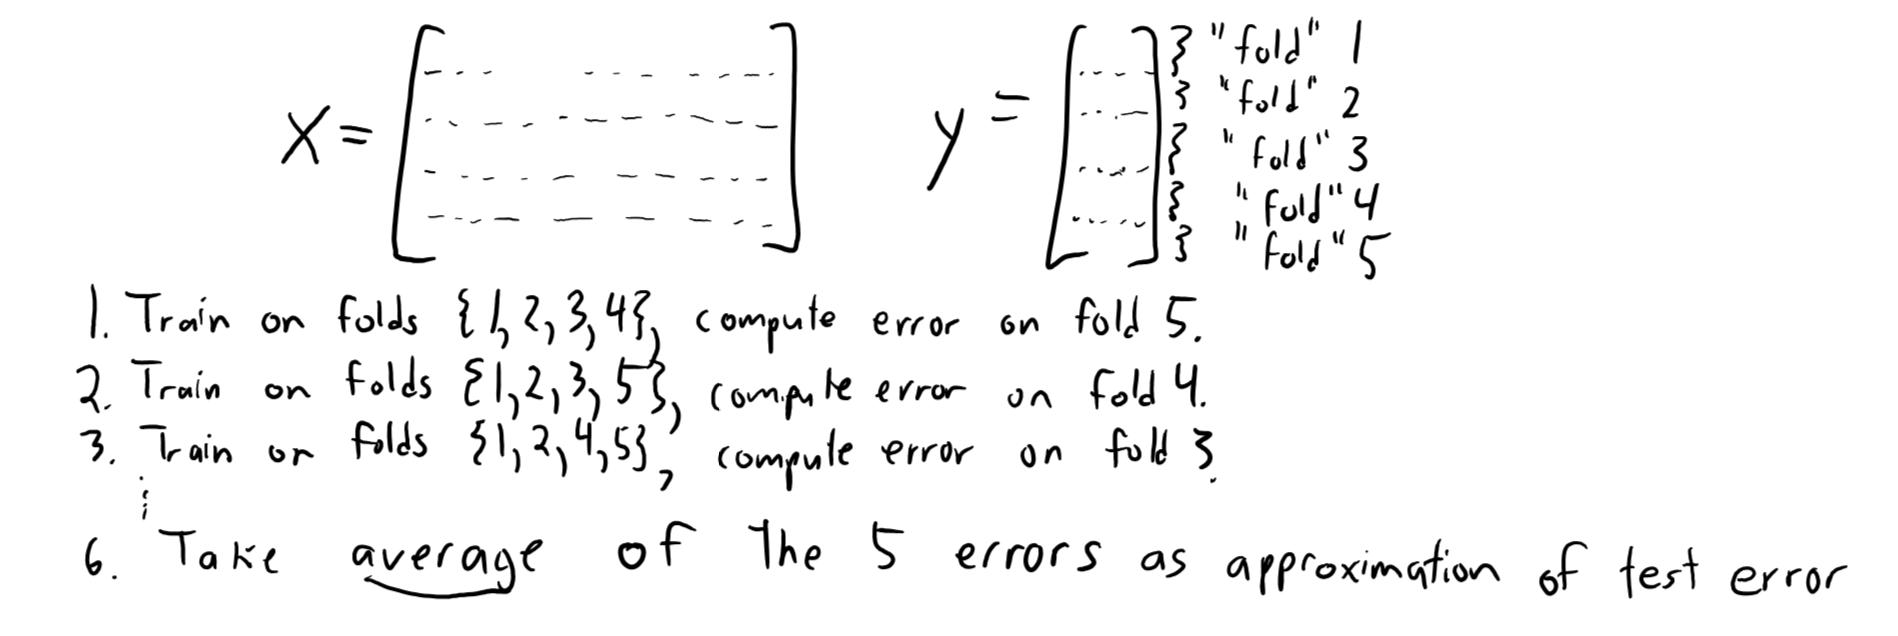
\includegraphics[width = 6in]{Pic11}
	\caption{Cross-validation example}
\end{figure}

\subsubsection*{Cross-validation Pseudocode}
\textsl{To choose depth}:
\begin{lstlisting}[tabsize=3]
for depth in 1:20:
	compute cross validation score
return depth with highest score
\end{lstlisting}
\textsl{To compute 5-fold cross validation score}:
\begin{lstlisting}[tabsize=3]
for fold in 1:5:
	train 80% that doesn't include fold
	test on fold
return average test error
\end{lstlisting}
You can also take this idea further: \textbf{k-fold cross validation}
\begin{itemize}
	\item {\color{blue} 10 fold cross validation}: train on 90\% of data, test on the remaining 10\% (repeat 10 times, for each fold, and average)
	\item {\color{blue} Leave one out cross-validation}: train on all but one training example, repeat $ n $ times and average.
\end{itemize}
This gets {\color{OliveGreen} more accurate} but {\color{red} more expensive} with each fold

\subsection*{The "Best" Machine Learning Model}
As decision trees are not always the most accurate on the test error, we ask what is the {\color{OliveGreen} best machine learning model} \\ \\
An alternative measure of performance is the {\color{blue} generalization error}
\begin{itemize}
	\item Average error over all $ x_i $ vectors that are not seen in the training set
	\item “How well we expect to do for a completely unseen feature vector”
\end{itemize}
{\color{red} No free lunch theorem}:
\begin{itemize}
	\item There is no "best" model for achieving the best generalization error for every problem
	\item If model A generalizes better to new data than model B on one data set, there is another data set where model B works better.
\end{itemize}
This implies that we need to try out multiple models. In CPSC 340, we focus on {\color{blue} models that have been effective in many applications}.

\subsection*{Application: E-mail Spam Filtering}
\textbf{Obj:} We want to build a system that {\color{OliveGreen} detects spam emails}. Can this be formulated in the form of supervised learning? \\ \\
Procedure:
\begin{enumerate}
	\item Collect a large number of emails, and get users to label them.
	\item We can use ($ y_i = 1 $) if email $ i $ is spam, and ($ y_i = 0 $) otherwise
	\item Extract features in each email (like {\color{blue} bag of words})
	\begin{itemize}[label=$ \cdot $]
		\item ($ x_{ij} = 1 $) if email $ i $ has word/phrase $ j $, ($ x_{ij} = 0 $) otherwise
	\end{itemize}
\end{enumerate}
\subsubsection*{Feature representation for Spam}
Are there better features than bag of words?
\begin{itemize}[label=-]
	\item We add {\color{blue} bigrams} (sets of two words)
	\begin{itemize}
		\item “CPSC 340”, “wait list”, “special deal”.
	\end{itemize}
	\item Or {\color{blue} tri-grams} (sets of three words)
	\begin{itemize}
		\item “Limited time offer”, “course registration deadline”, “you’re a winner”.
	\end{itemize}
	\item We might include the sender domain
	\begin{itemize}
		\item $ < $sender domain == “mail.com”$ > $
	\end{itemize}
	\item We might include regular expressions
	\begin{itemize}
		\item $ < $your first and last name$ > $
	\end{itemize}
\end{itemize}

\subsection*{Probabilistic Classifiers}
For years, the best spam filtering used naïve Baye's, which is a {\color{blue} probabilistic classifier} based on {\color{blue} Baye's rule}. It tends to {\color{blue} work well with bag of words}. \\ \\
\textbf{Probabilistic classifiers} model the conditional probability, $ P(y_i | x_i) $
\begin{itemize}[label=$ \cdot $]
	\item If a message has words $ x_i $ what is the probability that the message is spam?
\end{itemize}
Classify it as follows (classify it as spam if {\color{OliveGreen} probability of spam is higher than not spam}):
\begin{lstlisting}[tabsize=4]
	if (P(y[i] = "spam" | x[i]) > P(y[i] = "not spam" | x[i]))
		return "spam"
	else:
		return "not spam"
\end{lstlisting}
To model conditional probability, {\color{blue} Naïve Baye's} uses {\color{blue} Baye's rule}:
\begin{align*}
	P(y_i = \text{"spam"} | x_i) = \frac{P(x_i | y_i = \text{"spam"})P(\text{"spam"})}{P(x_i)}
\end{align*}
So we need to figure out 3 types of terms:
\begin{enumerate}
	\item {\color{blue} Marginal probability $ P(y_i) $} that and e-mail is spam
	\item {\color{blue} Marginal probability $ P(x_i) $} that an e-mail has the {\color{OliveGreen} set of words $ x_i $}
	\item {\color{blue} The conditional probability $ P(x_i | y_i) $} that {\color{OliveGreen} a spam email has the words $ x_i $}
\end{enumerate}
\textbf{Definitions of the terms:}
\begin{itemize}
	\item {\color{OliveGreen} $ P(y_i = \text{"spam"}) $} is the probability that a random email is spam. This is very easy to approximate from the data ({\color{blue} use proportion of emails that are spam}):
	{\color{blue}
	\begin{align*}
	P(y_i = \text{"spam"}) = \frac{\text{\# of spam messages}}{\text{\# of total messages}}
	\end{align*}}
	\item {\color{OliveGreen} $ P(x_i) $ is the probability that a random email has features $ x_i $}. {\color{red} This is hard to approximate}: for '$ d $' words {\color{red} we need to collect $ 2^d $ "coupons":}
	{\color{blue}
		\begin{align*}
		P(x_i) = \frac{\text{\# e-mails with features } x_i}{\text{\# of total messages}}
		\end{align*}}
	However, we can ignore it, since naïve Baye's returns "spam" if:
	\begin{align*}
	P(y_i = \text{"spam"} | x_i) &> P(y_i = \text{"not spam"} | x_i) \\
	\intertext{This means that:}
	\frac{P(x_i | y_i = \text{"spam"})P(\text{"spam"})}{P(x_i)} &> \frac{P(x_i | y_i = \text{"not spam"})P(\text{"not spam"})}{P(x_i)} \\
	\intertext{Multiplying by P(x_i) on both sides yields:}
	P(x_i | y_i = \text{"spam"})P(\text{"spam"}) &> P(x_i | y_i = \text{"not spam"})P(\text{"not spam"})
	\end{align*}
	\item {\color{OliveGreen} $ P(x_i|y_i=\text{"spam"}) $ is the probability that spam has features $ x_i $}. {\color{red} This is also hard to approximate}.
	{\color{blue}
		\begin{align*}
		P(x_i|y_i=\text{"spam"}) = \frac{\text{\# of spam messages with features } x_i}{\text{\# of spam messages}}
		\end{align*}}
\end{itemize}
\subsection*{Naïve Baye's}
Naïve Baye's makes a {\color{red} big assumption} to make things easier. Namely:
\begin{align*}
{\color{red} P(\text{hello = 1, vicodin = 0, 340 = 1} | \text{spam})} \approx {\color{blue}P(\text{hello = 1} | \text{spam})P(\text{vicodin = 0} | \text{spam})P(\text{340 = 1} | \text{spam})}
\end{align*}
This means that we assume that all features $ x_i $ are {\color{blue} independent given label $ y_i $}. Here:
\begin{itemize}
	\item Once you know it's spam, the probability of "vicodin" doesn't depend on "340".
	\item This is definitely not true, but a good approximation.
\end{itemize}
{\color{OliveGreen} Now only simple quantities are needed, like $ P(\text{"vicodin" = 0} | y_i\text{"spam"}) $.}:
{\color{blue}
	\begin{align*}
	P(\text{"vicodin" = 0} | y_i\text{"spam"}) = \frac{\text{\# of messages with "vicodin"}}{\text{total \# of messages}}
\end{align*}}



\end{document}